\documentclass[10pt, conference, compsocconf]{IEEEtran} %\documentclass[10pt, conference, compsocconf]{IEEEtran} %\documentclass[conference]{IEEEtran}%%\documentclass{llncs}
\usepackage{algorithm}
\usepackage{algpseudocode}
\usepackage{graphicx} 
\usepackage{subfig}
\usepackage{multirow}
\usepackage{tikz}
\usetikzlibrary{fit,positioning}
\usetikzlibrary{arrows}
\usetikzlibrary{calc}
\usepackage{url}
\usepackage{amsmath}
\usepackage{cleveref}

%\setlength{\parskip}{0pt}

\let\OLDthebibliography\thebibliography
\renewcommand\thebibliography[1]{
  \OLDthebibliography{#1}
  \setlength{\parskip}{0pt}
  \setlength{\itemsep}{0pt plus 0.3ex}
}

% Commands for Latin abbrevs, trailing slash is needed so that latex knows
% the final "." is not the end of a sentence.
\newcommand{\ie}{\textit{i.e.}\ }
\newcommand{\cf}{\textit{c.f.}\ }
\newcommand{\eg}{\textit{e.g.}\ }
\newcommand{\etal}{\textit{et al.}\ }
\newcommand{\etc}{etc.\ }

% End of integrals
\renewcommand{\d}{\;\mathrm{{d}}}


\begin{document}
\title{Scheduling Workflows onto Power-Constrained VMs}
\author{
\IEEEauthorblockN{David Shepherd, Ilia Pietri, Rizos Sakellariou}
\IEEEauthorblockA{School of Computer Science, University of Manchester, UK}
}

\maketitle

\begin{abstract}
With energy consumption being an issue of growing concern in large-scale cloud data centers, providers may wish to impose restrictions on the power usage of the hosts.
This raises the challenge of operating cloud resources under power limits which may vary over time.
Motivated by such a constraint, this paper considers the problem of scheduling scientific workflows in an environment where the number of VMs available is limited by a time-varying power cap.
A simple scheduling algorithm for such cases is proposed and experimentally evaluated.
\end{abstract}

\section{Introduction and Problem Description} %(workflows, scheduling, power cap)
\label{sec:intr-probl-descr}

Cloud computing platforms offer a flexible environment to provide user resources on demand.
However, the scale of existing cloud data centers may lead to high energy consumption, making electricity cost a significant element in their operation.
To manage such costs cloud providers may set power budgets~\cite{zhang2011capping}, which in turn may lead to power caps for specific users or applications.
This implies that the latter will have to adjust their demands accordingly and limit the number of VMs they use to the extent that they do not exceed the power cap.

%Power consumption is an increasing concern to be addressed in modern computing systems with the need for power management techniques arising in order to reduce power usage of the hosts. Among these, power capping is a mechanism used to constrain the power consumed by the hosts up to a certain limit \cite{kansal2010virtual}. To achieve this, power consumption is controlled by adjusting the number of operating hosts and their power management properties, e.g. CPU frequency \cite{fan2007power,bailey2014adaptive}. Cloud computing platforms offer a flexible environment to adjust the cloud resources according to the constraints dynamically by providing VM elasticity. The number of the VMs that can be assigned to the hosts may range depending on the power budget limit and power caps can be seen as a constraint that limits the number of VMs to be used for the execution of applications. However, the number of used VMs affects application performance as independent jobs can be executed in parallel. Depending on the power budget, the number of the VMs can be adjusted to optimise application performance. For example, an extra number of VMs can be allocated for the execution of parallel jobs when the power budget increases or deallocated when the power budget decreases postponing the execution of several jobs. 

This paper focuses on scheduling under a power cap in scientific workflow applications.
Scientific workflows \cite{deelmanbook} consist of inter-related tasks with data dependencies between them.
They can be modelled as a Directed Acyclic Graph (DAG) where the nodes represent the computational tasks and edges represent the data dependencies between them.
We assume that information on task runtime and data transfer is known and users are interested in (dynamically) maximizing the number of VMs provisioned to take advantage of the inherent parallelism in the workflow structure.
As the power budget limits the number of VMs that can be provisioned over time the problem that arises is how to schedule tasks onto VMs while taking into account fluctuations in the number of available VMs.
This paper suggests a scheduling algorithm to address this problem.

In contrast to related work making elaborate assessments of the power/performance correlation, such as \cite{bailey2014adaptive}, we use a simple power model and focus instead on the scheduling challenge.
We assume that a single class of VMs is available, and that they each have fixed power consumption (\ie no dynamic voltage or frequency scaling).


\section{The Algorithm}

As mentioned in \cref{sec:intr-probl-descr}, we assume that only a single type of VM with fixed power consumption is available.
Thus the number of VMs available is determined by the power cap: we allow the use of as many VMs as possible while remaining below the cap.
So the problem is reduced to scheduling jobs on a time-varying number of VMs.

Our algorithm is based on the well known Heterogeneous Earliest Finish Time (HEFT) scheduling algorithm \cite{Topcuoglu2002heft}.
HEFT is a static, heuristic scheduling algorithm.
It operates in two steps.
First the tasks are sorted by their upward rank, a combination of factors based on the job's mean computation time (over the available VMs), mean communication time, and the upward rank of its successors in the workflow DAG.
Second the tasks are scheduled, in the above order, to the VM that results in the earliest finish time for that job.
Due to space constraints we refer to the paper \cite{Topcuoglu2002heft} for details of the HEFT algorithm.

In standard HEFT initially all VMs are available at all times, and portions of time on the VMs are occupied by jobs as the algorithm progresses.
In our power-capped modification we instead begin with some portions of VM time occupied by dummy jobs at times when there is insufficient power to run that VM.
Following this initial modification of the available slots the algorithm proceeds as standard HEFT.
The key observation is that this does not interfere with the running of HEFT except to prevent jobs from being scheduled to unavailable VMs.
The pseudocode for this algorithm is given in \cref{alg:power-capped-heft}.

Note that, despite the name, our algorithm currently assumes homogeneous VMs.
However the algorithm could be easily extended for heterogeneous VMs by the addition of some heuristic for determining which VMs provide optimal performance per watt for the given tasks.

Also note that the power cap is only ``theoretically'' enforced: if jobs overrun it may be violated unless the VM is killed and a new schedule is calculated.
This inability to adapt to changing circumstances is a limitation of static scheduling algorithms.

\begin{algorithm}
  \begin{algorithmic}[1]
    \State Determine the number of VMs available over time within the power cap
    \State Schedule dummy jobs at times when VMs are unavailable
    \State Run HEFT with the modified initial schedule

    % \State Compute computation costs of tasks and commumcation costs of edges.
    % \State Compute upward rank for all tasks
    % \State Sort tasks in non-increasing order of upward rank
    % \For{task $t$ in \texttt{ranked\_tasks}}
    %     \For{VM $v$ in \texttt{VM\_list}}
    %         \State Compute $\texttt{EFT}(t, v)$
    %     \EndFor
    %     \State Assign task $t$ to VM $v'$ that minimises $\texttt{EFT}(t, v')$
    % \EndFor

  \end{algorithmic}
  \caption{Power-capped HEFT scheduling algorithm.}
  \label{alg:power-capped-heft}
\end{algorithm}

\section{Experimental Evaluation}

In order to evaluate its performance on large workflows the proposed algorithm was implemented within the cloud workflow simulator \cite{CloudWorkflowSimulator,malawski2012cost}.
Performance is tested on synthetic workflow data corresponding to real scientific applications generated using WorkflowGenerator \cite{WorkflowGenerator,Bharathi2008}.

The performance of the power-capped HEFT algorithm was compared to a simple first-come-first-served (FCFS) scheduling approach, where jobs are scheduled to the first available VM in the order that the jobs are ready (\ie when all predecessors in the workflow DAG are complete).

For these experiments the power cap $P(t)$ is chosen to be a simple piecewise-constant function of time.
It begins with power $P_0$, drops to power $P_0/2$ at time $\tau/3$, then jumps back to power $P_0$ at time $2\tau/3$.
The values of $P_0$ and $\tau$ are chosen based on the workflow as:
\begin{equation}
  P_0 =, \quad \tau =,
\end{equation}
which correspond to $P_0$ approximately ??ds, and $\tau$ approximately the makespan.

The makespan (total run time), $T$, is normalised by $T' = \alpha \int_0^T P(t) \d t$ where $\alpha$ is the instructions executed per unit of power consumption for the VMs.
$T'$ corresponds to the optimal makespan if all available power was used, ignoring the fact that VMs use discrete amounts of power and that jobs take a discrete amount of time.

??ds Figures show...

??ds some analysis of the results...

\begin{figure}
  \centering
  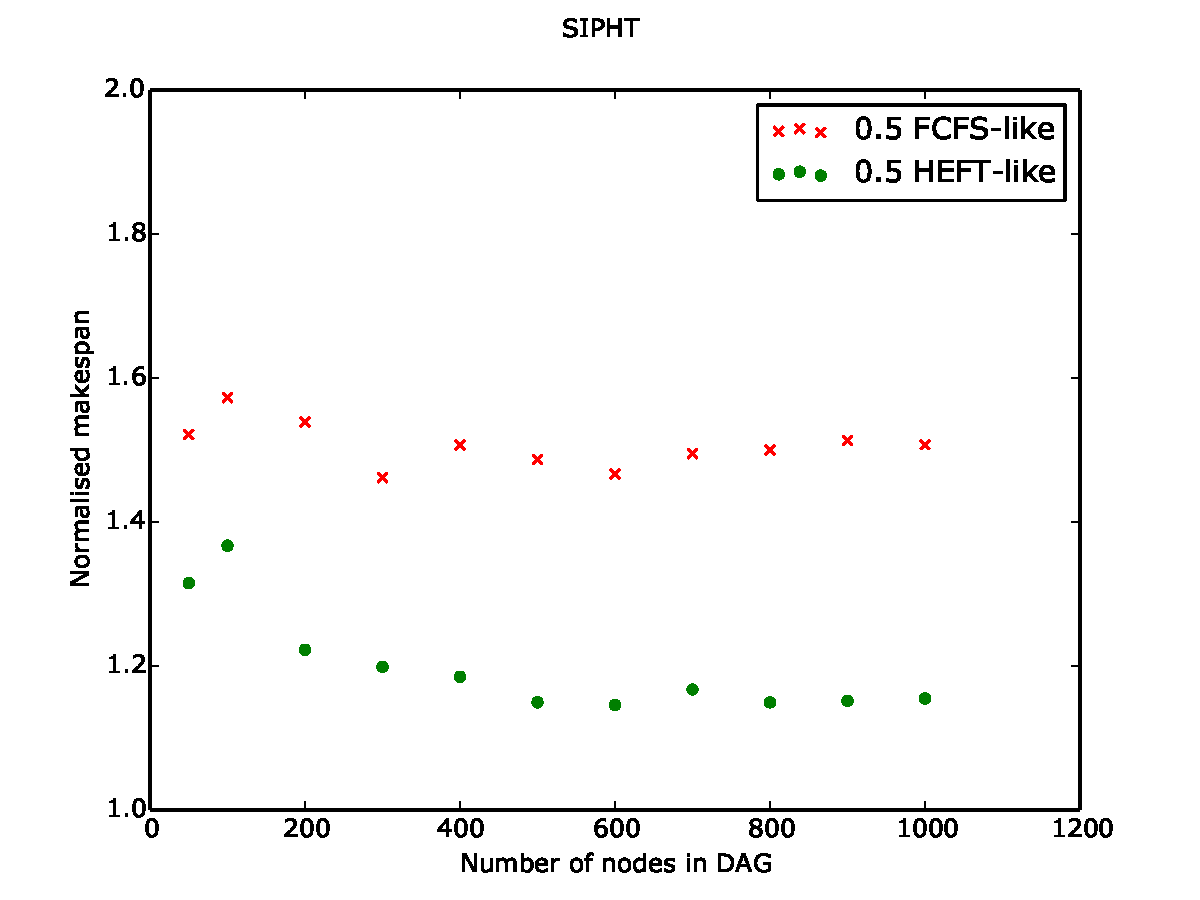
\includegraphics[width=\columnwidth]{{{images/schedule-length-ratio-SIPHT}}}
  \caption{}
  \label{fig:placeholder}
\end{figure}

\begin{figure}
  \centering
  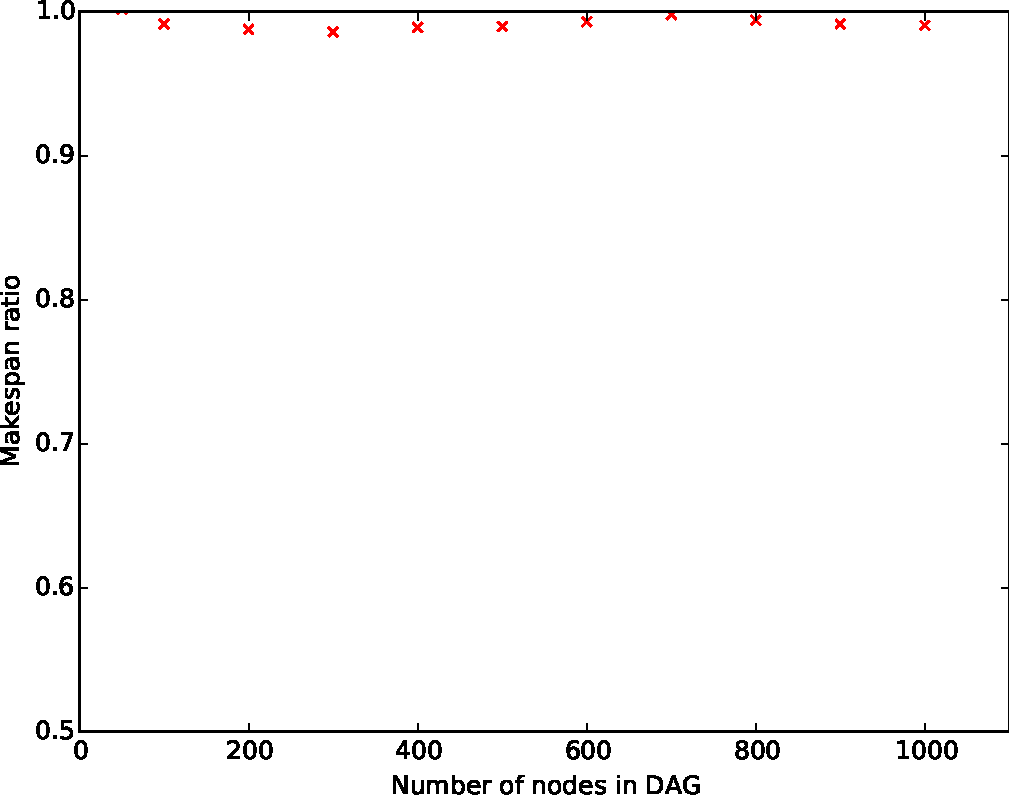
\includegraphics[width=\columnwidth]{{{images/schedule-length-ratio-MONTAGE}}}
  \caption{}
  \label{fig:placeholder1}
\end{figure}

\section{Conclusion}

??ds here goes the conclusion (4-5 lines should be enough)
%This paper addressed the problem of resource provisioning and workflow scheduling under power constraints. It proposed an algorithm that determines the number of VMs to be provisioned for the workflow execution and schedule the tasks onto the available VMs so that the power budget is met.

\bibliographystyle{IEEEtran}
\bibliography{references}



\end{document}


